\documentclass[t]{beamer}

\subtitle{Applications of the Division Algorithm}

\usepackage{amsthm,amsmath,amsfonts,hyperref,graphicx,color,multicol,soul}
\usepackage{enumitem,tikz,tikz-cd,setspace,mathtools}

%%%%%%%%%%
%Beamer Template Customization
%%%%%%%%%%
\setbeamertemplate{navigation symbols}{}
\setbeamertemplate{theorems}[ams style]
\setbeamertemplate{blocks}[rounded]

\definecolor{Blu}{RGB}{43,62,133} % UWEC Blue
\setbeamercolor{structure}{fg=Blu} % Titles

%Unnumbered footnotes:
\newcommand{\blfootnote}[1]{%
	\begingroup
	\renewcommand\thefootnote{}\footnote{#1}%
	\addtocounter{footnote}{-1}%
	\endgroup
}

%%%%%%%%%%
%TikZ Stuff
%%%%%%%%%%
\usetikzlibrary{arrows}
\usetikzlibrary{shapes.geometric}
\tikzset{
	smaller/.style={
		draw,
		regular polygon,
		regular polygon sides=3,
		fill=white,
		node distance=2cm,
		minimum height=1in,
		line width = 2pt
	}
}
\tikzset{
	smsquare/.style={
		draw,
		regular polygon,
		regular polygon sides=4,
		fill=white,
		node distance=2cm,
		minimum height=1in,
		line width = 2pt
	}
}


%%%%%%%%%%
%Custom Commands
%%%%%%%%%%

\newcommand{\C}{\mathbb{C}}
\newcommand{\quats}{\mathbb{H}}
\newcommand{\N}{\mathbb{N}}
\newcommand{\Q}{\mathbb{Q}}
\newcommand{\R}{\mathbb{R}}
\newcommand{\Z}{\mathbb{Z}}

\newcommand{\ds}{\displaystyle}

\newcommand{\fn}{\insertframenumber}

\newcommand{\id}{\operatorname{id}}
\newcommand{\im}{\operatorname{im}}
\newcommand{\lcm}{\operatorname{lcm}}
\newcommand{\Aut}{\operatorname{Aut}}
\newcommand{\Inn}{\operatorname{Inn}}

\newcommand{\blank}[1]{\underline{\hspace*{#1}}}

\newcommand{\abar}{\overline{a}}
\newcommand{\bbar}{\overline{b}}
\newcommand{\cbar}{\overline{c}}

\newcommand{\nml}{\unlhd}

%%%%%%%%%%
%Custom Theorem Environments
%%%%%%%%%%
\theoremstyle{definition}
\newtheorem{exercise}{Exercise}
\newtheorem{question}[exercise]{Question}
\newtheorem{warmup}{Warm-Up}
\newtheorem*{exa}{Example}
\newtheorem*{disc}{Group Discussion}
\newtheorem*{recall}{Recall}
\renewcommand{\emph}[1]{{\color{blue}\texttt{#1}}}

\definecolor{Gold}{RGB}{237, 172, 26}
%Statement block
\newenvironment{statementblock}[1]{%
	\setbeamercolor{block body}{bg=Gold!20}
	\setbeamercolor{block title}{bg=Gold}
	\begin{block}{\textbf{#1.}}}{\end{block}}
\newenvironment{goldblock}{%
	\setbeamercolor{block body}{bg=Gold!20}
	\setbeamercolor{block title}{bg=Gold}
	\setbeamertemplate{blocks}[shadow=true]
	\begin{block}{}}{\end{block}}
\newenvironment{defn}{%
	\setbeamercolor{block body}{bg=gray!20}
	\setbeamercolor{block title}{bg=violet, fg=white}
	\setbeamertemplate{blocks}[shadow=true]
	\begin{block}{\textbf{Definition.}}}{\end{block}}
\newenvironment{nb}{%
	\setbeamercolor{block body}{bg=gray!20}
	\setbeamercolor{block title}{bg=teal, fg=white}
	\setbeamertemplate{blocks}[shadow=true]
	\begin{block}{\textbf{Note.}}}{\end{block}}
\newenvironment{blockexample}{%
	\setbeamercolor{block body}{bg=gray!20}
	\setbeamercolor{block title}{bg=Blu, fg=white}
	\setbeamertemplate{blocks}[shadow=true]
	\begin{block}{\textbf{Example.}}}{\end{block}}
\newenvironment{blocknonexample}{%
	\setbeamercolor{block body}{bg=gray!20}
	\setbeamercolor{block title}{bg=purple, fg=white}
	\setbeamertemplate{blocks}[shadow=true]
	\begin{block}{\textbf{Non-Example.}}}{\end{block}}
\newenvironment{thm}[1]{%
	\setbeamercolor{block body}{bg=Gold!20}
	\setbeamercolor{block title}{bg=Gold}
	\begin{block}{\textbf{Theorem #1.}}}{\end{block}}


%%%%%%%%%%
%Custom Environment Wrappers
%%%%%%%%%%
\newcommand{\exer}[1]{
	\begin{exercise}
		#1
	\end{exercise}
}
\newcommand{\exam}[1]{
\begin{blockexample}
	#1
\end{blockexample}
}
\newcommand{\nexam}[1]{
\begin{blocknonexample}
	#1
\end{blocknonexample}
}
\newcommand{\enumarabic}[1]{
	\begin{enumerate}[label=\textbf{\arabic*.}]
		#1
	\end{enumerate}
}
\newcommand{\enumalph}[1]{
	\begin{enumerate}[label=(\alph*)]
		#1
	\end{enumerate}
}
\newcommand{\bulletize}[1]{
	\begin{itemize}[label=$\bullet$]
		#1
	\end{itemize}
}
\newcommand{\circtize}[1]{
	\begin{itemize}[label=$\circ$]
		#1
	\end{itemize}
}
\newcommand{\slide}[1]{
	\begin{frame}{\fn}
		#1
	\end{frame}
}
\newcommand{\slidec}[1]{
\begin{frame}[c]{\fn}
	#1
\end{frame}
}
\newcommand{\slidet}[2]{
	\begin{frame}{\fn\ - #1}
		#2
	\end{frame}
}


\newcommand{\startdoc}{
		\title{Math 341: Classical Number Theory}
		\author{Mckenzie West}
		\date{Last Updated: \today}
		\begin{frame}
			\maketitle
		\end{frame}
}

\newcommand{\topics}[2]{
	\begin{frame}[c]{\insertframenumber}
		\begin{block}{\textbf{Last Section.}}
			\begin{itemize}[label=--]
				#1
			\end{itemize}
		\end{block}
		\begin{block}{\textbf{This Section.}}
			\begin{itemize}[label=--]
				#2
			\end{itemize}
		\end{block}
	\end{frame}
}

\begin{document} 
	\startdoc
	
	\topics{
		% This time
		\item Using Sage via BGSC
		\item The Division Algorithm
	}
	{
		\item Consequences of the Division Algorithm
		\item Divisibility Rules
	}

\slide{
	\exam{\textbf{Motivation from Historical Text.}
		
		From the \underline{Ganitasara Sangraha}, a text written by Mahaviracharya, a Jain mathematician in approximately 850 A.D.
		
		\begin{goldblock}
			There were 63 heaps of plantain fruit put together and 7 single fruits. They were equally distributed among 23 travelers leaving no remainder. What is one possible number of fruits in each pile?
		\end{goldblock}
		\begin{center}
			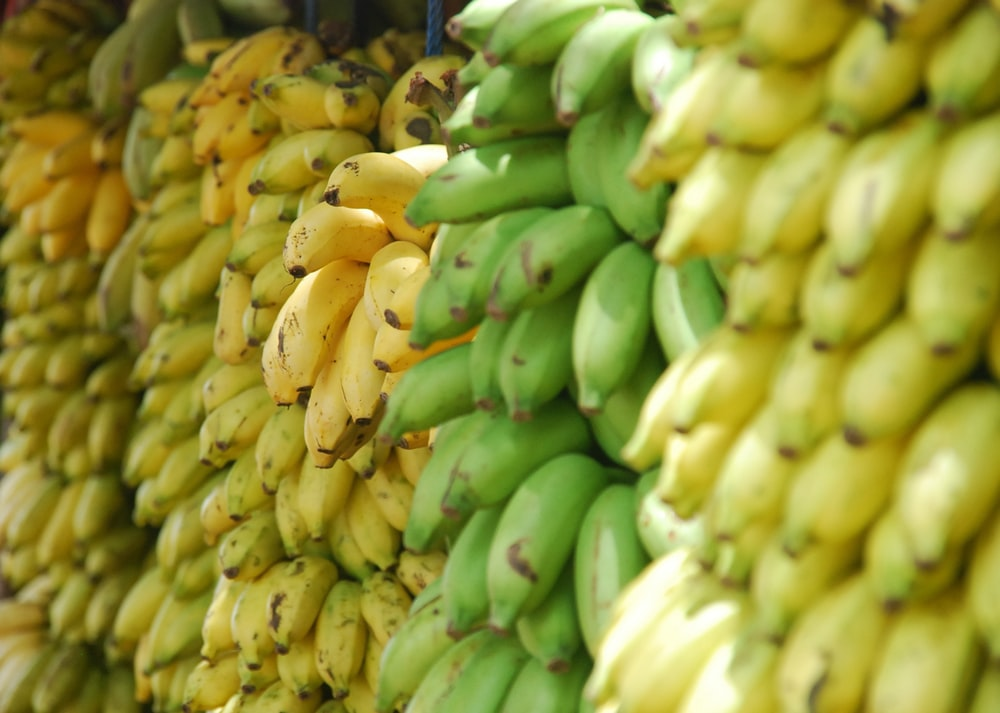
\includegraphics[width=1.5in]{plantains}
		\end{center}
	}
}
\slide{
	\begin{block}{\textbf{Goal.}}
		Really we're trying to find positive integers $x$ and $y$ such that 
			\[63x+7=23y.\]
			
		Or, in the form we'll be using:
			\[-63x+23y=7.\]
	\end{block}
	\begin{nb}
		This is called a \emph{Diophantine equation} and we'll learn how to solve these next week.
	\end{nb}
}
\slide{
	\begin{statementblock}{The Division Algorithm}
		Given integers $a$ and $b$ with $b>0$, there exist unique integers $q$ and $r$ satisfying
			\[a=qb+r\quad 0\leq r<b.\]
		We call $q$ the \emph{quotient} and $r$ the \emph{remainder} in the division of $a$ by $b$
	\end{statementblock}
	\begin{statementblock}{Corollary}
		If $a$ and $b$ are integers with $b\neq 0$, then there exist unique integers $q$ and $r$ satisfying
			\[a=qb+r\quad 0\leq r<|b|.\]
	\end{statementblock}
}
\slide{
	\begin{exercise}
		Let's take $b=-4$ and some $a$ values \blank{.25in}, \blank{.25in}, and \blank{.25in}.
		
		Then using the division algorithm, we have
		
		\[\blank{.25in}=\blank{.25in}\cdot(-4)+\blank{.25in}\]\vfill
		\[\blank{.25in}=\blank{.25in}\cdot(-4)+\blank{.25in}\]\vfill	
		\[\blank{.25in}=\blank{.25in}\cdot(-4)+\blank{.25in}\]
	\end{exercise}
}
\slide{
	\begin{nb}
		The Division Algorithm allows us to classify integers into a finite number of cases for example \emph{even} ($2q+0$) and \emph{odd} ($2q+1$).
	\end{nb}
	\begin{exercise}
		Show that for all integers $a$, we have $a^2$ is either a multiple of 4 or one more than a multiple of 4.
	\end{exercise}
}
\slide{
	\begin{exercise}
		Show that for all integers $a$, if $a$ is odd then $a^2$ is of the form $8a+1$.
	\end{exercise}
}
\slide{
	\begin{exercise}
		Show that $\ds\frac{a(a^2+2)}{3}$ is an integer for all $a\in\Z$.
	\end{exercise}
}
\slide{
	\begin{exercise}
		Show that the cube of an integer is of the form $7k$ or $7k\pm 1$.
	\end{exercise}
}
\slide{
	\begin{exercise}
		Show that if an integer is simultaneously a square and a cube, then it must be of the form $7k$ or $7k+ 1$.
	\end{exercise}
}
\slide{
	\begin{nb}
		Divisibility corresponds to checking if $r=0$ in the division algorithm.
	\end{nb}
	\begin{exercise}
		Show that in every sequence of 3 consecutive integers, one of the numbers is divisible by $3$.
	\end{exercise}
}
\slide{
	\begin{exercise}
		Fill in the divisibility rules: An integer $n$ is divisible
		\bulletize{\setlength{\itemsep}{2em}
			\item by 2 if:
			\item by 3 if:
			\item by 4 if:
			\item by 5 if:
			\item by 6 if:
		}
	\end{exercise}
}
\slide{
\begin{exercise}
	Fill in the divisibility rules: An integer $n$ is divisible
	\bulletize{\setlength{\itemsep}{3em}
		\item by 8 if:
		\item by 9 if:
		\item by 10 if:
		\item by 11 if:
	}
\end{exercise}
}
\end{document}

